%%%%%%%%%%%%%%%%%%%%%%%%%%%%%%%%%%%%%%%%%
% Short Sectioned Assignment LaTeX Template Version 1.0 (5/5/12)
% This template has been downloaded from: http://www.LaTeXTemplates.com
% Original author:  Frits Wenneker (http://www.howtotex.com)
% License: CC BY-NC-SA 3.0 (http://creativecommons.org/licenses/by-nc-sa/3.0/)
%%%%%%%%%%%%%%%%%%%%%%%%%%%%%%%%%%%%%%%%%

%----------------------------------------------------------------------------------------
%	PACKAGES AND OTHER DOCUMENT CONFIGURATIONS
%----------------------------------------------------------------------------------------

\documentclass[paper=a4, fontsize=11pt]{scrartcl} % A4 paper and 11pt font size

% ---- Entrada y salida de texto -----

\usepackage[T1]{fontenc} % Use 8-bit encoding that has 256 glyphs
\usepackage[utf8]{inputenc}
\usepackage{hyperref}
%\usepackage{fourier} % Use the Adobe Utopia font for the document - comment this line to return to the LaTeX default

% ---- Idioma --------

\usepackage[spanish, es-tabla]{babel} % Selecciona el español para palabras introducidas automáticamente, p.ej. "septiembre" en la fecha y especifica que se use la palabra Tabla en vez de Cuadro

% ---- Otros paquetes ----

\usepackage{url} % ,href} %para incluir URLs e hipervínculos dentro del texto (aunque hay que instalar href)
\usepackage{amsmath,amsfonts,amsthm} % Math packages
%\usepackage{graphics,graphicx, floatrow} %para incluir imágenes y notas en las imágenes
\usepackage{graphics,graphicx, float} %para incluir imágenes y colocarlas

% Para hacer tablas comlejas
%\usepackage{multirow}
%\usepackage{threeparttable}

%\usepackage{sectsty} % Allows customizing section commands
%\allsectionsfont{\centering \normalfont\scshape} % Make all sections centered, the default font and small caps

\usepackage{fancyhdr} % Custom headers and footers
\pagestyle{fancyplain} % Makes all pages in the document conform to the custom headers and footers
\fancyhead{} % No page header - if you want one, create it in the same way as the footers below
\fancyfoot[L]{} % Empty left footer
\fancyfoot[C]{} % Empty center footer
\fancyfoot[R]{\thepage} % Page numbering for right footer
\renewcommand{\headrulewidth}{0pt} % Remove header underlines
\renewcommand{\footrulewidth}{0pt} % Remove footer underlines
\setlength{\headheight}{13.6pt} % Customize the height of the header

\numberwithin{equation}{section} % Number equations within sections (i.e. 1.1, 1.2, 2.1, 2.2 instead of 1, 2, 3, 4)
\numberwithin{figure}{section} % Number figures within sections (i.e. 1.1, 1.2, 2.1, 2.2 instead of 1, 2, 3, 4)
\numberwithin{table}{section} % Number tables within sections (i.e. 1.1, 1.2, 2.1, 2.2 instead of 1, 2, 3, 4)

\setlength\parindent{0pt} % Removes all indentation from paragraphs - comment this line for an assignment with lots of text

\newcommand{\horrule}[1]{\rule{\linewidth}{#1}} % Create horizontal rule command with 1 argument of height


%----------------------------------------------------------------------------------------
%	TÍTULO Y DATOS DEL ALUMNO
%----------------------------------------------------------------------------------------

\title{	
\normalfont \normalsize 
\textsc{\textbf{Ingeniería de Servidores (2016-2017)} \\ Grado en Ingeniería Informática \\ Universidad de Granada} \\ [25pt] % Your university, school and/or department name(s)
\horrule{0.5pt} \\[0.4cm] % Thin top horizontal rule
\huge Memoria Práctica 4 \\ % The assignment title
\horrule{2pt} \\[0.5cm] % Thick bottom horizontal rule
}

\author{Sergio Samaniego Martínez} % Nombre y apellidos

\date{\normalsize\today} % Incluye la fecha actual

%----------------------------------------------------------------------------------------
% DOCUMENTO
%----------------------------------------------------------------------------------------

\begin{document}

\maketitle % Muestra el Título

\newpage %inserta un salto de página

\tableofcontents % para generar el índice de contenidos


\newpage

%----------------------------------------------------------------------------------------
%	Cuestión 1
%----------------------------------------------------------------------------------------

\section{Cuestión 1}
\subsection{\Large Seleccione, instale y ejecute uno, comente los resultados. Atención: no es lo mismo un benchmark que una suite, instale un benchmark.}
Primero vamos a instalar Phoronix. 
Para ello basta con ejecutar el comando : \$ sudo apt-get install phoronix-test-suite

Una vez instalado como nos indica la página referenciada, para que instale correctamente las dependencias necesarias hay que cambiar algunas cosas en el archivo que usa phoronix para poder instalar dichas dependencias, que se encuentra en /usr/share/phoronix-test-suite/pts-core/external-test-dependencies/scripts/install-ubuntu-packages.sh  \cite{phoronix}

Hecho esto, mostramos la lista disponible de test.

\begin{figure}[H] %con el [H] le obligamos a situar aquí la figura
	\centering
	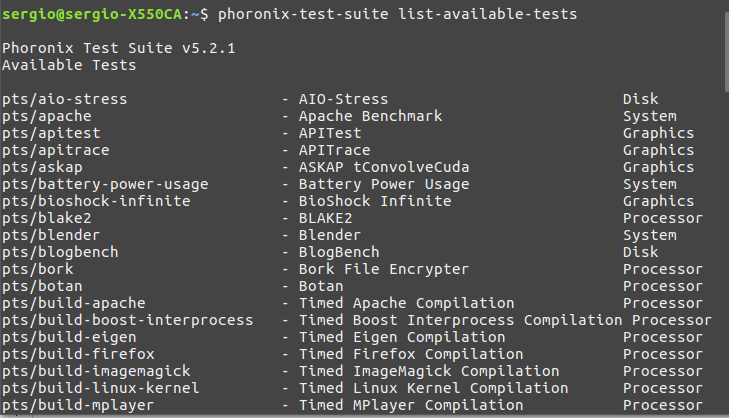
\includegraphics[scale=0.5]{imagenes/list-test.png}  %el parámetro scale permite agrandar o achicar la imagen. En el nombre de archivo puede especificar directorios
	\caption{Muestra del comando para instalar apache benchmark, el cual ya tenía instalado}
\end{figure}

Elegimos uno, en nuestro caso compress-gzip y lo instalamos.

\begin{figure}[H] %con el [H] le obligamos a situar aquí la figura
	\centering
	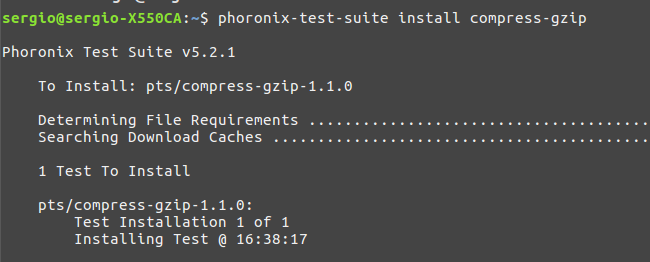
\includegraphics[scale=0.5]{imagenes/install-gzip.png}  %el parámetro scale permite agrandar o achicar la imagen. En el nombre de archivo puede especificar directorios
	\caption{Comando para instalar el test gzip}
\end{figure}

Una vez instalado, lo ejecutamos.

\begin{figure}[H] %con el [H] le obligamos a situar aquí la figura
	\centering
	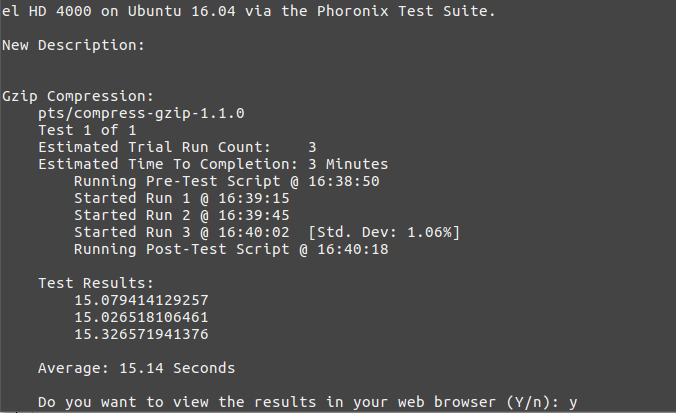
\includegraphics[scale=0.5]{imagenes/run-gzip.png}  %el parámetro scale permite agrandar o achicar la imagen. En el nombre de archivo puede especificar directorios
	\caption{Ejecución del test gzip}
\end{figure}

Terminada la ejecución, vemos los resultados en la página \url{www.openbenchmarking.org}

\begin{figure}[H] %con el [H] le obligamos a situar aquí la figura
	\centering
	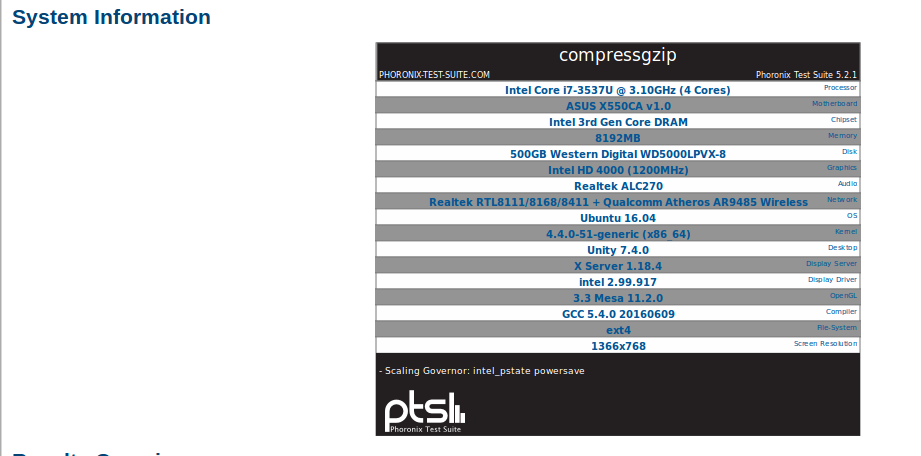
\includegraphics[scale=0.5]{imagenes/system-information.png}  %el parámetro scale permite agrandar o achicar la imagen. En el nombre de archivo puede especificar directorios
	\caption{En la página nos aparecen los detalles del sistema}
\end{figure}


\begin{figure}[H] %con el [H] le obligamos a situar aquí la figura
	\centering
	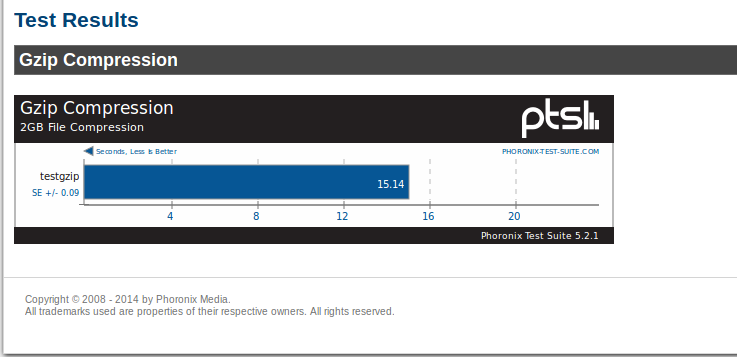
\includegraphics[scale=0.5]{imagenes/graphic-gzip.png}  %el parámetro scale permite agrandar o achicar la imagen. En el nombre de archivo puede especificar directorios
	\caption{Gráfica con los resultados del test realizado.}
\end{figure}


\section{Cuestión 2}
\subsection{\Large De los parámetros que le podemos pasar al comando ¿Qué significa -c 5 ? ¿y -n 100?}

La opción -c hace referencia a la concurrencia, por lo tanto, si le pasamos como parámetro -c 5, significa que se va a ejecutar concurrentemente 5 solicitudes a la vez.
En el caso de -n significa el número de solicitudes que se le van a realizar al servidor, por lo tanto significa que le haremos 100 solicitudes al servidor. \cite{ab}

\subsection{\Large Monitorice la ejecución de ab contra alguna máquina (cualquiera) ¿cuántas “tareas” crea ab en el cliente?}

Para hacer la prueba instalo apache benchmark en mi máquina anfitrión:

\begin{figure}[H] %con el [H] le obligamos a situar aquí la figura
	\centering
	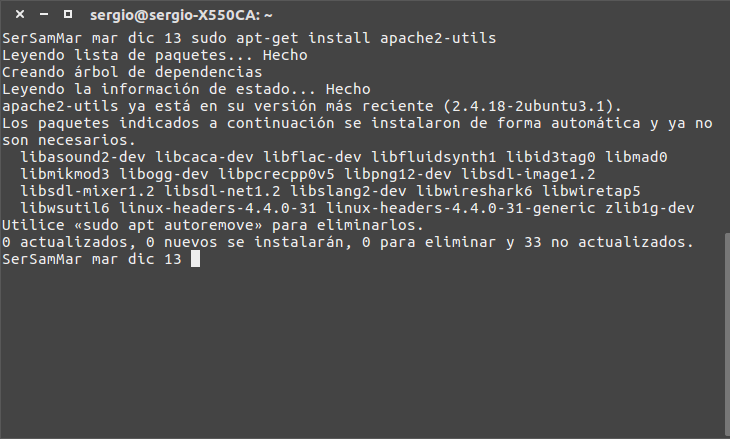
\includegraphics[scale=0.5]{imagenes/instalo-ab.png}  %el parámetro scale permite agrandar o achicar la imagen. En el nombre de archivo puede especificar directorios
	\caption{Muestra del comando para instalar apache benchmark, el cual ya tenía instalado}
\end{figure}

Una vez instalado, vamos a ejecutar apache benchmark sobre nuestra máquina virtual de Ubuntu Server, para ello miramos su direccón IP con ifconfig, y vemos que es 192.168.56.192

Para monitorizarlo, vamos a quitarle concurrencia y a añadirle más solicitudes para que tarde más tiempo en ejecutar el benchmark.

Una vez hecho esto, ejecutamos Apache Benchmark y en otra terminal vemos el número de procesos creados con el comando "ps -af".

\begin{figure}[H] %con el [H] le obligamos a situar aquí la figura
	\centering
	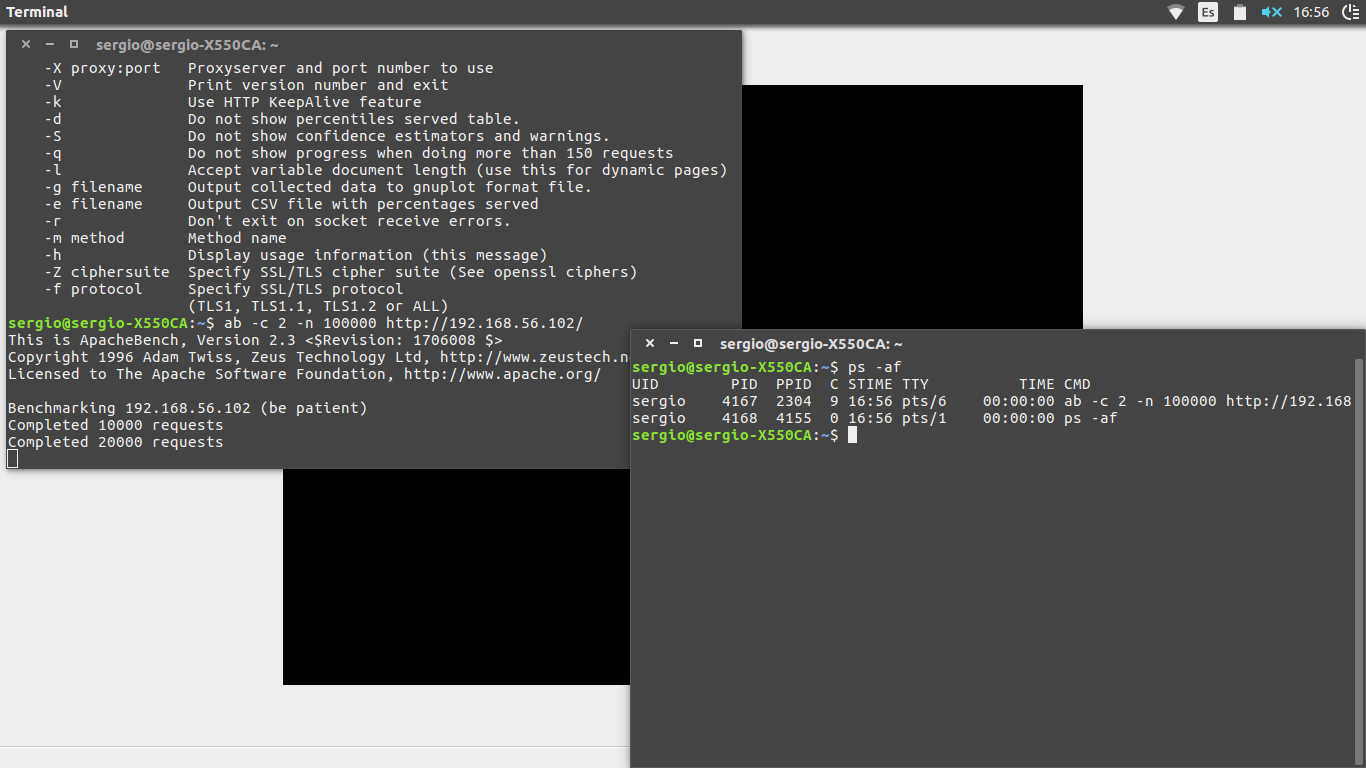
\includegraphics[scale=0.35]{imagenes/monitor-ab.png}  %el parámetro scale permite agrandar o achicar la imagen. En el nombre de archivo puede especificar directorios
	\caption{Comprobación del número de procesos que crea Apache Benchmark.}
\end{figure}

Como se ve en la figura, sólo se ha creado un proceso durante la ejecución del benchmark.


\section{Cuestión 3}

\subsection{Ejecute ab contra a las tres máquinas virtuales (desde el SO anfitrión a las máquina virtuales de la red local) una a una (arrancadas por separado).¿Cuál es la que proporciona mejores resultados? Muestre y coméntelos. (Use como máquina de referencia Ubuntu Server para la comparativa). }

Para que la comparación entre las tres máquinas virtuales sea real, hemos cambiado en las 3 la página html por defecto, para que así no haya diferencias debido a que en una deba cargar imágenes o simplemente más contenido.

Ejecución de Apache Benchmark sobre Ubuntu Server
\begin{figure}[H] %con el [H] le obligamos a situar aquí la figura
	\centering
	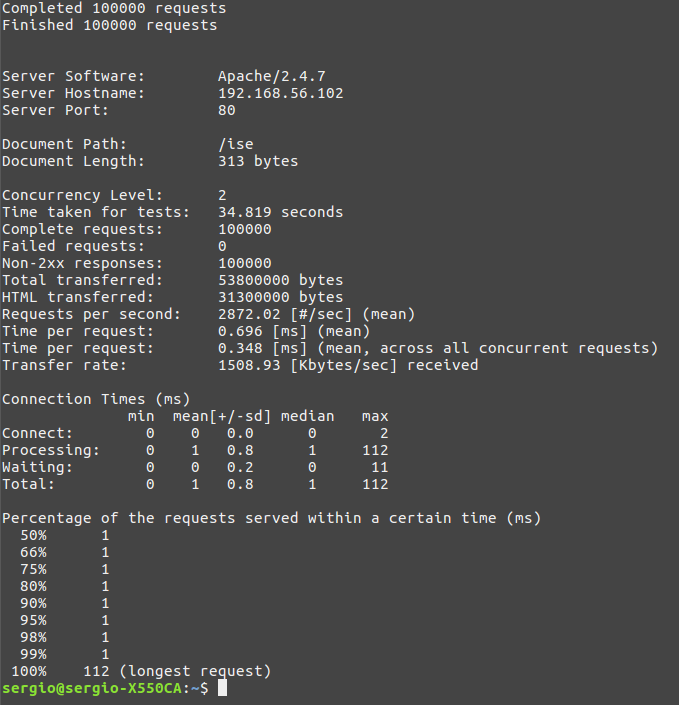
\includegraphics[scale=0.5]{imagenes/ab-us.png}  %el parámetro scale permite agrandar o achicar la imagen. En el nombre de archivo puede especificar directorios
	\caption{Monitorización de Apache Benchmark sobre Ubuntu Server}
\end{figure}
Como vemos en los resultados obtenidos, el tiempo medio de solicitud es 0.348 ms, el número medio de solicitudes por segundo son 2872.02 y la velocidad transferida es 1508.93 Kbytes/segundo

\setlength{\parskip}{10pt}

Ejecución de Apache Benchmark sobre Windows Server.
\begin{figure}[H] %con el [H] le obligamos a situar aquí la figura
	\centering
	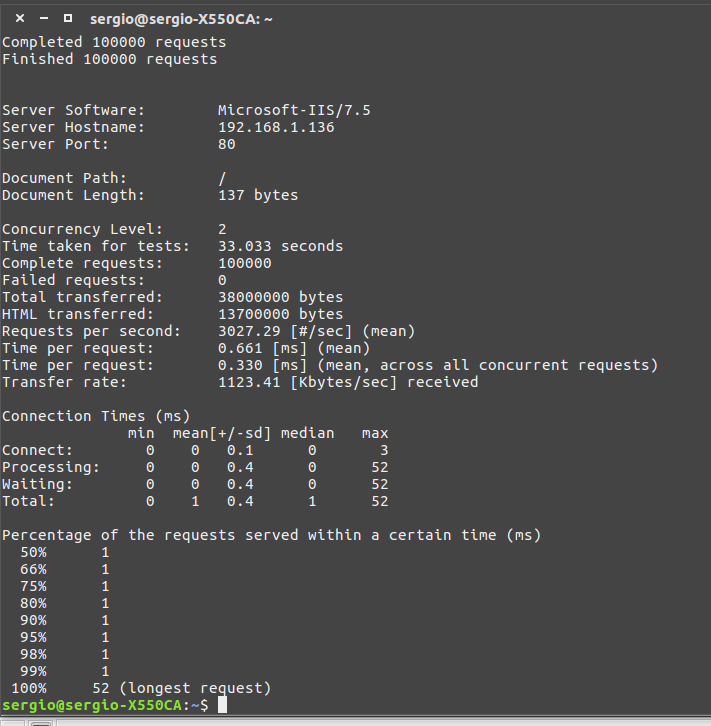
\includegraphics[scale=0.5]{imagenes/ab-ws.png}  %el parámetro scale permite agrandar o achicar la imagen. En el nombre de archivo puede especificar directorios
	\caption{Monitorización de Apache Benchmark sobre Windows Server}
\end{figure}
Los resultados de Windows Server como se ve, son 0.330 ms como tiempo medio de solicitud, una media de 3027.29 solicitudes por segundo y una velocidad media de transferencia de 1123.41 Kbytes/segundo.

\setlength{\parskip}{10pt}

Ejecución de Apache Benchmark sobre CentOS.

\begin{figure}[H] %con el [H] le obligamos a situar aquí la figura
	\centering
	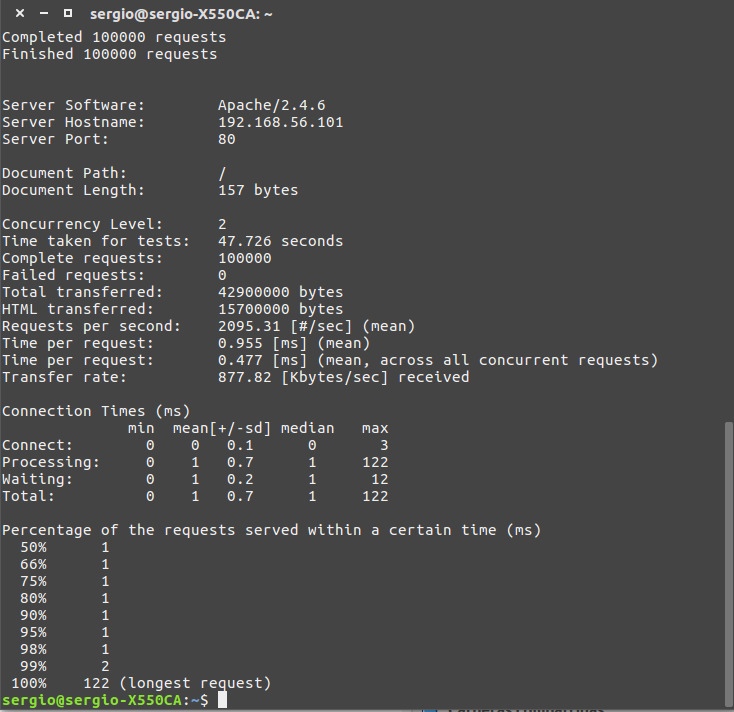
\includegraphics[scale=0.5]{imagenes/ab-centos.png}  %el parámetro scale permite agrandar o achicar la imagen. En el nombre de archivo puede especificar directorios
	\caption{Monitorización de Apache Benchmark sobre CentOS}
\end{figure}

En CentOs obtenemos como resultados, 0.477 ms de tiempo medio de solicitud, una media de 2095.31 peticiones por segundo y una velocidad media de transferencia de 877.82 KBytes/segundo.


\setlength{\parskip}{20pt}

Como podemos comprobar con los resultados obtenidos en cada una de las ejecuciones, 
Ubuntu Server es el sistema con mayor velocidad de transferencia, pero no podemos decir lo mismo en cuanto al tiempo medio de respuesta y al número de peticiones por segundo donde en ambas cosas el sistema operativo que obtiene mejores resultados es Windows Server. 
\\Entre los tres sistemas el que peor resultados obtiene es CentOs.


%------------------------------------------------

\section{Cuestión 4}

\subsection{\Large Instale y siga el tutorial en http://jmeter.apache.org/usermanual/build-web-test-plan.html realizando capturas de pantalla y comentándolas. En vez de usar la web de jmeter, haga el experimento usando sus máquinas virtuales ¿coincide con los resultados de ab?}

Lo primero que debemos hacer será instalar jmeter.
Esto es un paso sencillo ya que nos basta con realizar un comando como mostramos en la figura 5.1

\begin{figure}[H] %con el [H] le obligamos a situar aquí la figura
	\centering
	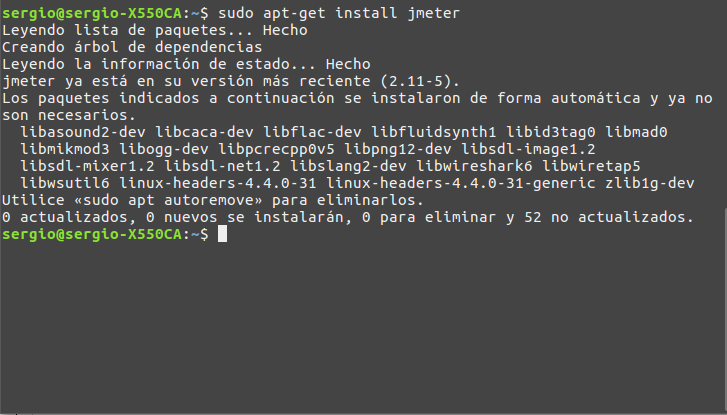
\includegraphics[scale=0.5]{imagenes/install-jmeter.png}  %el parámetro scale permite agrandar o achicar la imagen. En el nombre de archivo puede especificar directorios
	\caption{Comando de instalación de jmeter.}
\end{figure}

En mi caso ya está instalado.
\\El siguiente paso que haremos será ejecutarlo, para ello escribimos en la terminal jmeter y se ejecutará.

\begin{figure}[H] %con el [H] le obligamos a situar aquí la figura
	\centering
	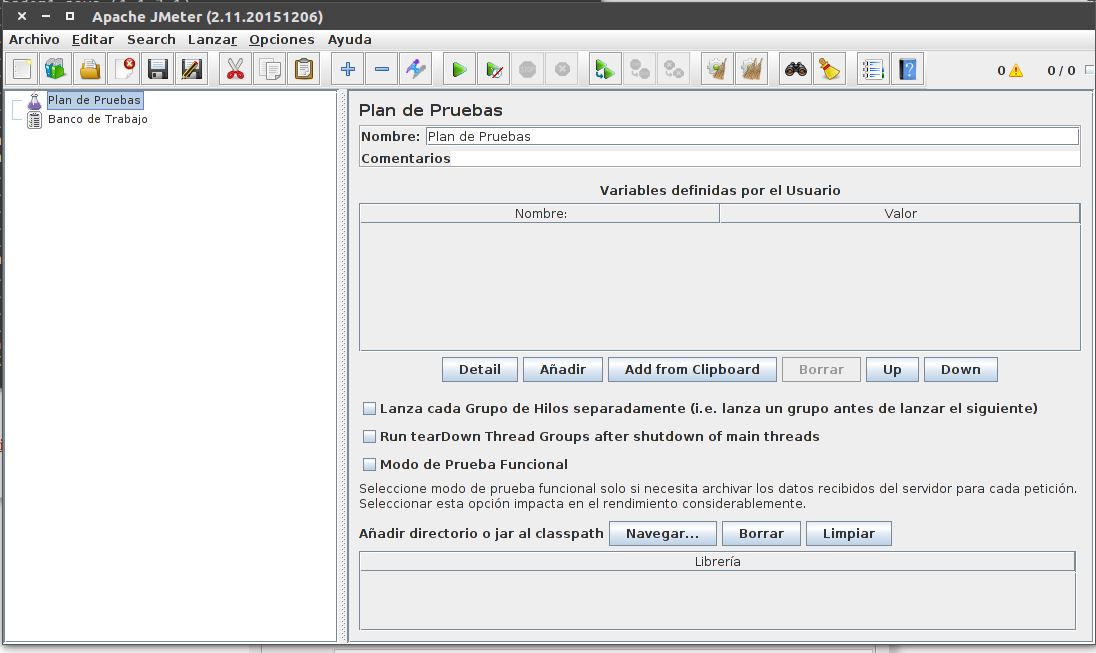
\includegraphics[scale=0.35]{imagenes/jmeter-1.png}  %el parámetro scale permite agrandar o achicar la imagen. En el nombre de archivo puede especificar directorios
	\caption{Ejecución de jmeter.}
\end{figure}

Una vez ejecutado, lo que hacemos será primero añadir usuarios para realizar las peticiones.
\\Para ello damos click derecho en Plan de Pruebas->Añadir->Hilos(Usuario)->Grupo de Hilos.

\begin{figure}[H] %con el [H] le obligamos a situar aquí la figura
	\centering
	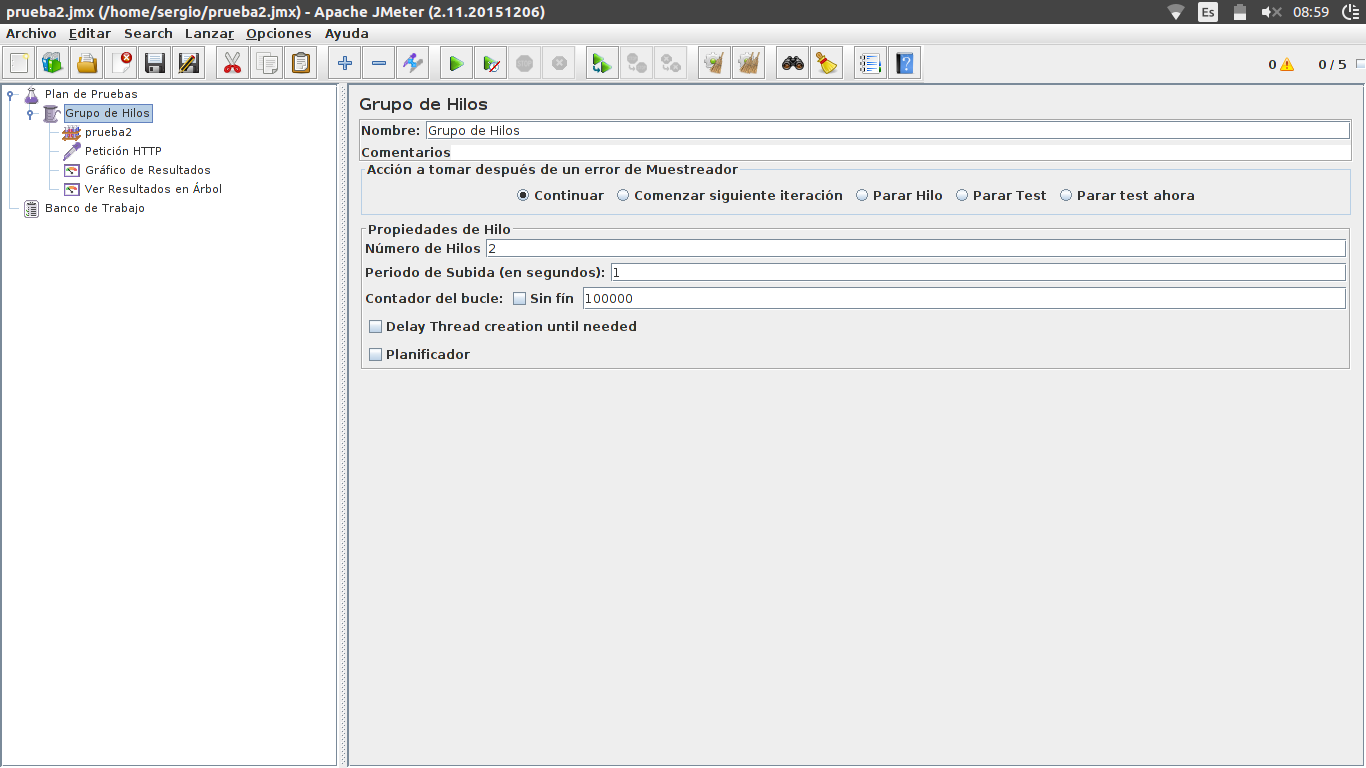
\includegraphics[scale=0.35]{imagenes/grupo-hilos.png}  %el parámetro scale permite agrandar o achicar la imagen. En el nombre de archivo puede especificar directorios
	\caption{Creación de grupo de usuarios.}
\end{figure}

Los valores por defecto al crear el grupo de usuarios es:
\\El número de hilos que será lo que nosotros interpretaremos como usuarios será igual a 1, nosotros queremos que haya varios usuarios a la vez realizando peticiones, por eso le pondré 2.
\\El periodo de subida será igual a 1, este parámetro hace referencia a la diferencia de tiempo que habrá entre que acabe un usuario y empiece otro a realizar una nueva petición.
\\Contador de bucle será igual a 1, el cual nos dirá cuantas veces vamos a repetir el test, nosotros realizaremos el test 100000 veces.

\setlength{\parskip}{10pt}

Ya creados los usuarios, vamos a realizar el test HTTP.
Para ello, hacemos click derecho sobre el grupo de usuarios->Añadir->Muestreador->Petición HTTP \cite{jmeter}

\begin{figure}[H] %con el [H] le obligamos a situar aquí la figura
	\centering
	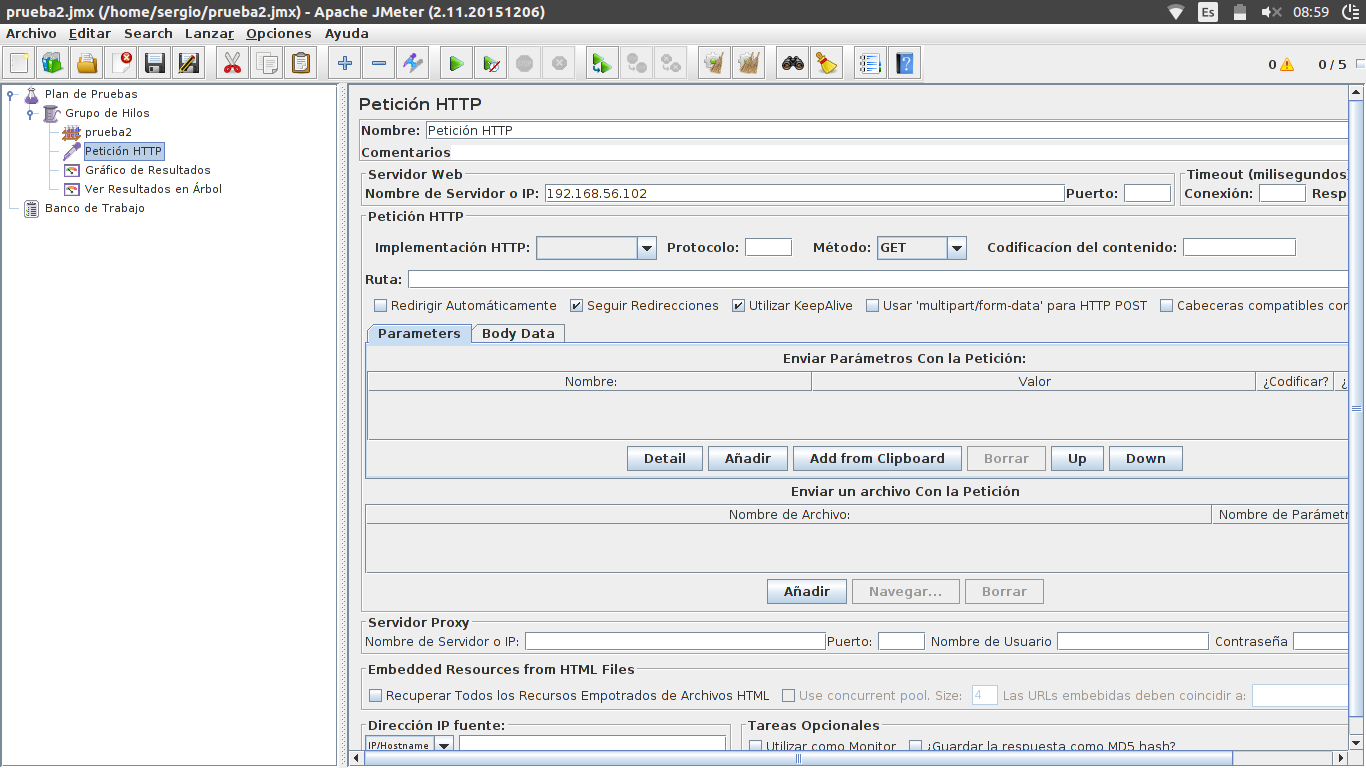
\includegraphics[scale=0.35]{imagenes/peticion-us.png}  %el parámetro scale permite agrandar o achicar la imagen. En el nombre de archivo puede especificar directorios
	\caption{Valores por defecto de petición HTTP.}
\end{figure}

En la IP, introduciremos la IP de nuestra máquina virtual, en este caso, la de Ubuntu Server. Esta página debe ser la misma que se ejecutó con ApacheBenchmark para poder hacer una comparación real.

Una vez ya ejecutado, mostramos los resultados, en este caso con un gráfico.

\begin{figure}[H] %con el [H] le obligamos a situar aquí la figura
	\centering
	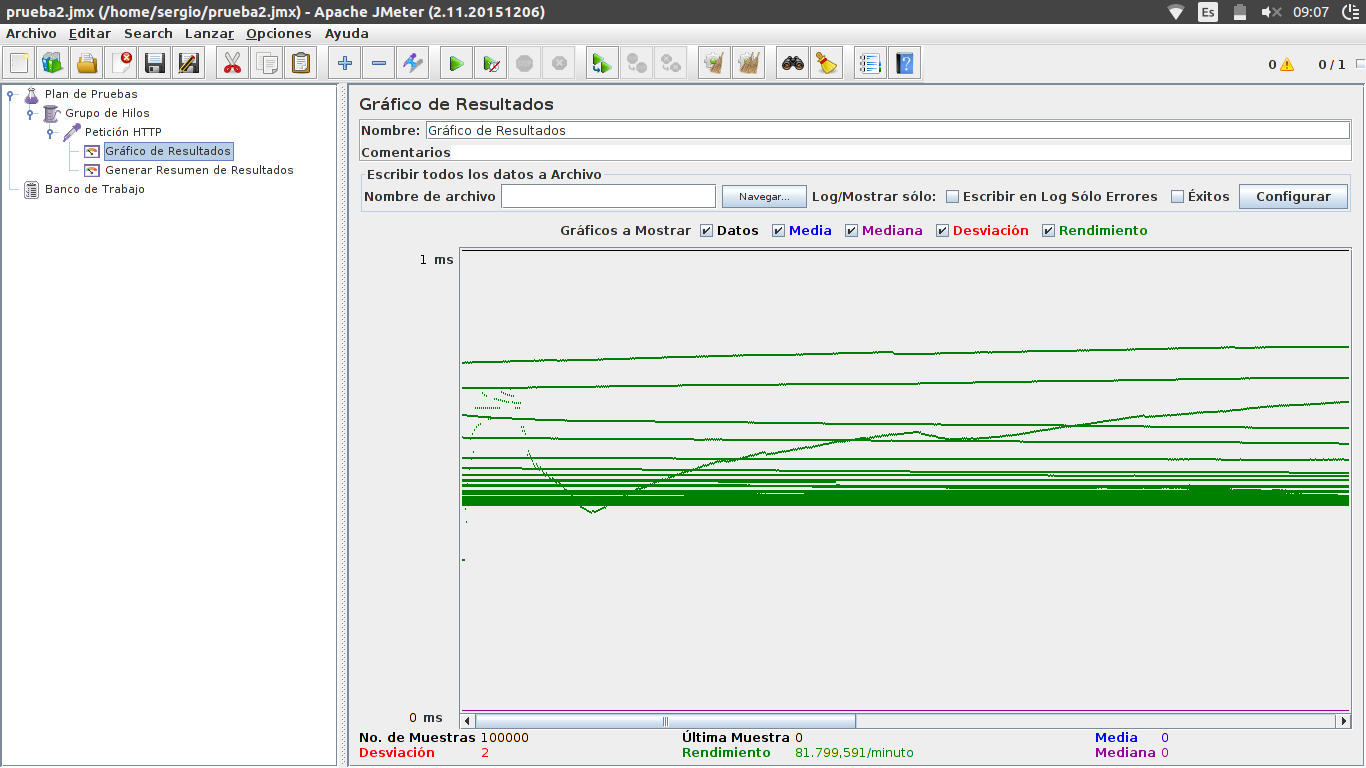
\includegraphics[scale=0.35]{imagenes/grafico.png}  %el parámetro scale permite agrandar o achicar la imagen. En el nombre de archivo puede especificar directorios
	\caption{Grafico de resultados de petición de HTTP.}
\end{figure}

Como podemos ver en el gráfico, la media de tiempo por cada petición está un poco por debajo de 0,5 ms y en ApacheBenchmark nos salía alrededor de los 0,4 ms, por lo que podemos ver que ambas mediciones se asemejan.
En cuanto a la media de peticiones, Jmeter nos da una media de 81799,59 / minuto, mientras que ApacheBenchmark nos daba 2872peticiones/segundo, que si lo pasamos a minutos para poder compararlas, con ApacheBenchmark nos saldría una media de 172320 peticiones/segundo lo cual como vemos, difiere bastante es algo más que el doble que nos da Jmeter.









%------------------------------------------------

\section{Cuestión 5}

\subsection{\Large Programe un benchmark usando el lenguaje que desee. El benchmark debe incluir:\\ 1) Objetivo del benchmark. \\2) Métricas (unidades, variables, puntuaciones, etc.) \\3) Instrucciones para su uso. \\4) Ejemplo de uso analizando los resultados.}

El Benchmark que vamos a usar es procBench.

El objetivo de dicho benchmark es el de medir el rendimiento del procesador realizando distintas operaciones matemáticas.

Este benchMark está en ensamblador y en cuanto a las medidas que utiliza, usará:
\begin{itemize}
	\item Velocidad de los registros: Medirá en MIPS la velocidad de los registros al añadir instrucciones, utilizando 1,2,3 o 4 registros.
	\item Test de lectura de memoria: EN este test se medirá la velocidad en MB/s de la lectura de memoria de distintos tamaños de buffer(4KBytes, 8KBytes, etc.).
	\item Generación: En este test se medirá la velocidad de generación en segundos de distintas operaciones como son la generación de números aleatorios, de la secuencia de fibonacci, etc.
	contenidos...
\end{itemize}

Para utilizar este benchmark, no hay más que descargarlo,\cite{procbench} y dependiendo del sistema operativo que estemos coriendo, tendremos un .exe para windows y un archivo ejecutable para linux.

En mi caso voy a modificar dicho benchmark debido a que quiero analizar la velocidad para generar las distintas secuencias que vienen por defecto, ya que ni la velocidad de lectura de memoria ni la de los registros me interesan.

Una vez modificado esto, para que sólo nos realice lo que queremos pasaremos a ejecutarlo.

\begin{figure}[H] %con el [H] le obligamos a situar aquí la figura
	\centering
	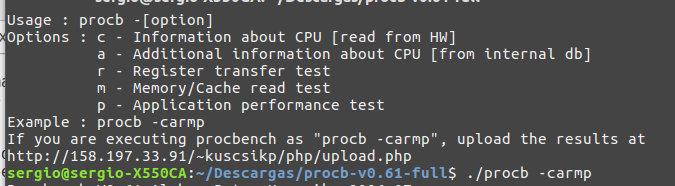
\includegraphics[scale=0.5]{imagenes/procb-info.png}  %el parámetro scale permite agrandar o achicar la imagen. En el nombre de archivo puede especificar directorios
	\caption{Información para ejecutar correctamente procbench}
\end{figure}

Para ejecutar el benchmark, lo que debemos hacer es añadirle alguno de estos parámetros, dependiendo de qué test queramos realizar.

Yo voy a realizar un test general, por lo que haré una ejecución en la cual le pasaré como parámetros todos aquellos que se muestran, como se ve al final de la figura 4.1.

Una vez ejecutado dicho benchmark, obtenemos los resultados.

\begin{figure}[H] %con el [H] le obligamos a situar aquí la figura
	\centering
	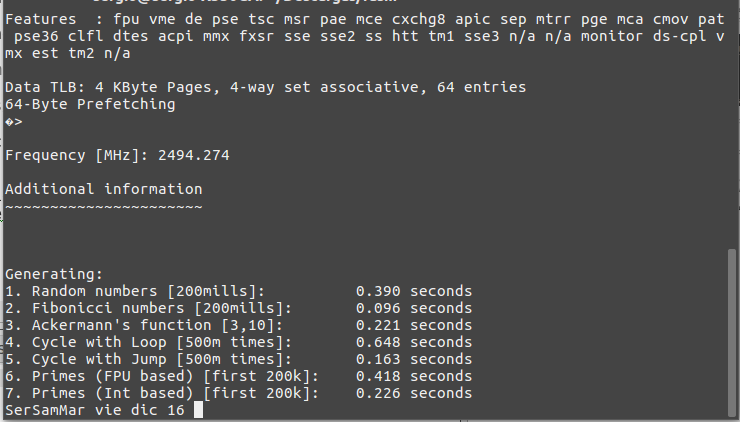
\includegraphics[scale=0.5]{imagenes/procbenc-run.png}  %el parámetro scale permite agrandar o achicar la imagen. En el nombre de archivo puede especificar directorios
	\caption{Información para ejecutar correctamente procbench}
\end{figure}

Como se ve en la figura4.2, tenemos sólamente las medidas de la generación de secuencias.

Para comprobar resultados, vamos a transferir el archivo ejecutable a la máquina virtual, esto lo haremos con scp.

\begin{figure}[H] %con el [H] le obligamos a situar aquí la figura
	\centering
	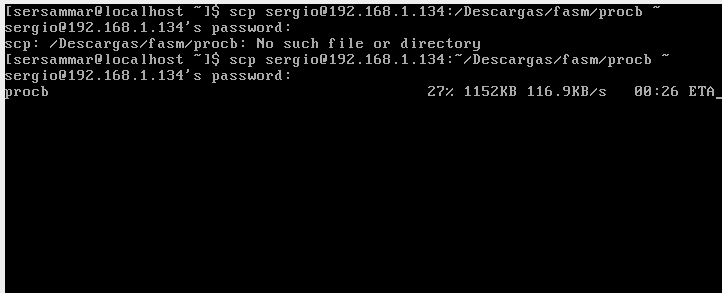
\includegraphics[scale=0.5]{imagenes/pasar-archivo.png}  %el parámetro scale permite agrandar o achicar la imagen. En el nombre de archivo puede especificar directorios
	\caption{Transferencia de archivo hacia la máquina virtual.}
\end{figure}

Una vez transferido lo ejecutamos y vemos los resultados.

\begin{figure}[H] %con el [H] le obligamos a situar aquí la figura
	\centering
	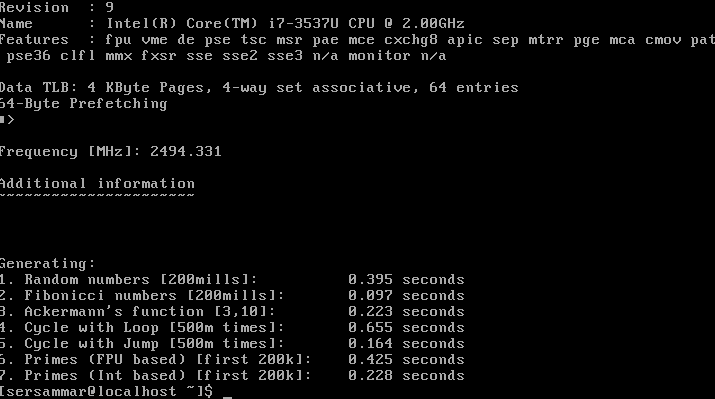
\includegraphics[scale=0.5]{imagenes/procb-centos.png}  %el parámetro scale permite agrandar o achicar la imagen. En el nombre de archivo puede especificar directorios
	\caption{Ejecución del benchmark sobre Centos.}
\end{figure}


Debido a que lo que estamos mirando es la CPU, al ser sobre el mismo pc, no importa que sea una máquina virtual, ya que la CPU seguirá siendo la misma, por eso los resultados son prácticamente idénticos.
Para ser listas generadas tan grandes el tiempo que tarda el procesador en generarlas podemos ver que es bastante pequeño, de lo que podemos deducir que nuestro procesador tiene una velocidad aceptable.


\newpage
\bibliography{citas} %archivo citas.bib que contiene las entradas 
\bibliographystyle{plain} % hay varias formas de citar

\end{document}
